\documentclass[12pt]{article}

\usepackage{sbc-template}
\usepackage{graphicx,url}
\usepackage[utf8]{inputenc}
\usepackage[brazil]{babel}
%\usepackage[latin1]{inputenc}  
     
\sloppy

\title{Arquitetura para Detecção de Postura Inadequada para Prevenção de Hipercifose Utilizando Arduino Lilypad}

\author{Ênio J. F. Júnior\inst{1}, Jonas S. Ramos\inst{1}, Hiel A. Rocha\inst{1} }

\address{Bacharelado em Ciência da Computação -- Instituto de Educação Superior\\ de Brasília
  (IESB) -- Brasília -- DF -- Brazil
  \email{\{juniorr452,jjonasramos\}@gmail.com,  hielrocha@outlook.com.br}
}

\begin{document} 

\maketitle
     
\begin{resumo} 
  Este artigo apresenta uma arquitetura para detecção de postura incorreta com o uso de componentes de Arduino e lógica fuzzy. O objetivo é notificar o usuário se a postura dele estiver incorreta para prevenir a hipercifose
\end{resumo}

\section{Introdução}

Ter uma postura correta é fundamental para evitar problemas na coluna e ter uma boa qualidade de vida. De acordo com \cite{cru:17}, segundo a OMS, a dor nas costas atinge cerca de 80\% da população mundial, sendo um dos motivos para isso a postura inadequada. Já outro levantamento aponta que dor nas costas foi uma das principais causas para afastamento no trabalho \cite{ig:17}.  

Além de, eventualmente, causar dor nas costas, a má postura pode de causar deformidades na coluna, como, por exemplo, a hipercifose, um agravamento da curvatura natural da coluna, como pode ser visto na Figura \ref{fig:example4}. 

\begin{figure}[ht]
\centering
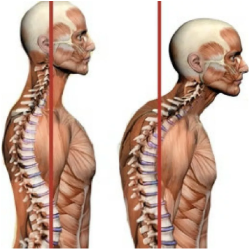
\includegraphics{fig4.png}
\caption{Cifose (esquerda) e hipercifose (direita) (Imagem: Vickyfisio)}
\label{fig:example4}
\end{figure}

Segundo Vidal, a cifose é “uma curvatura normal da coluna vertebral” \cite{vidal:17}. Já a hipercifose é “uma alteração nessa região da coluna que leva a um aumento da cifose normal, deixando os ombros projetados para frente e o dorso arredondado” \cite{vidal:17}. Uma das causas é a má postura, que pode acarretar dor nas costas.

Este projeto tem como objetivo utilizar os componentes de acelerômetro e o \textit{buzzer}, projetados especificamente para integração com tecidos, para detectar e notificar o usuário se sua postura está adequada ou não, a fim de prevenir futuros problemas na coluna.

O artigo está estruturado da seguinte maneira: na seção 2, está documentada a referência bibliográfica, com explicações sobre a técnica de inteligência artificial utilizada, o conceito de postura e os trabalhos correlatos; na seção 3, são apresentados a arquitetura do projeto e os conjuntos fuzzy utilizados.

\section{Revisão Bibliográfica}
\subsection{Lógica Fuzzy}
Ao contrário da lógica booleana, que permite apenas dois estados (ligado ou desligado, zero ou um), a lógica fuzzy se baseia em na ideia de conjuntos fuzzy, conjuntos esses que são caracterizados pelas funções de pertinência. Dentro de um sistema fuzzy, a entrada é fuzzificada, ou seja, transformada em graus de pertinência dos conjuntos fuzzy. A partir disso, é feita a inferência sobre esses valores e a defuzificação dos valores para se obter uma saída.

\subsection{Postura}
A postura, como conceituado por Teixeira (2011), Bricot (2001) e Kendall et al (1995), descrito por Fonseca, é "a resultante do conjunto de forças musculares que atuam continuamente para compensar o efeito da gravidade [...] possibilitando a manutenção da postura ereta"  \cite{fonseca:2015}. Como já definido por Vidal na seção 1, a hipercifose é uma alteração específica nessa estrutura, projetando o dorso para frente. A postura, então, fica comprometida, podendo levar a dores e outros problemas.
\subsection{Trabalhos Correlatos}
Em 2017, a camisa inteligente \textit{10ELEVEN9} \cite{colorfy:17} foi apresentada no site de financiamento coletivo \textit{Kickstarter}. A proposta era de proporcionar diversas funcionalidades com uma única peça vestível. Dentre elas, pode-se destacar o uso de um sensor de acelerômetro para detectar a postura do usuário e informá-lo, caso ela seja considerada incorreta. Por estar integrado junto ao sensor de batimentos cardíacos, o componente fica localizado na região peitoral. A descrição do projeto não especifica qual o algoritmo utilizado para considerar a postura correta ou incorreta.

\begin{figure}[ht]
\centering
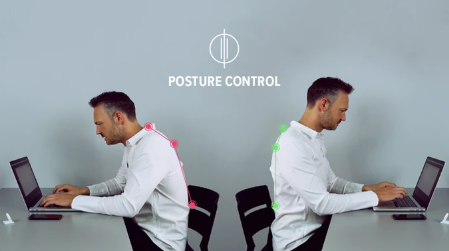
\includegraphics[width=.6\textwidth]{fig2.png}
\caption{Sistema de controle de postura do 10ELEVEN9}
\label{fig:example2}
\end{figure}

O trabalho \textit{Posture Correction with Wearable Electronics} \cite{rubow:08} teve, como objetivo, identificar a postura inadequada do usuário. Os componentes utilizados nesse projeto foram: Arduino Lilypad, dois acelerômetros e um módulo \textit{bluetooth} para receber dados dos sensores.

Quanto ao posicionamento dos componentes e algoritmos do projeto, os acelerômetros são posicionados na região dos ombros e o cosseno do ângulo entre os vetores gravitacionais dos sensores são calculados. O usuário é notificado por um som pelo módulo \textit{bluetooth} quando a diferença entre eles passa de um determinado limiar.

O estudo concluiu que o uso do módulo \textit{bluetooth}, bem como a bateria e regulador de voltagem, não seriam adequados, pois esses componentes não foram projetados especificamente para roupas. Inclusive, tais componentes precisaram ser acoplados a uma placa para então ser costurado na roupa, o que deixou o protótipo com aspecto esquisito.

\section{O Projeto}

\subsection{Tecnologias}

Para construir uma arquitetura de detecção de postura incorreta, foram utilizados os softwares e componentes de hardware: Arduino IDE; Arduino Lilypad; Acelerômetro e \textit{Buzzer}.

O Arduino IDE é um software que permite escrever programas para serem executados no dispositivo Arduino Lilypad. O sensor de acelerômetro e o \textit{buzzer} possibilitam obter os dados necessários para saber a postura e notificar o usuário, caso ela não esteja adequada.

\subsection{Arquitetura}

Um modelo da arquitetura proposta pode ser visualizado na Figura \ref{fig:example3}, que mostra a ligação entre o Lilypad e seus componentes. As cores das ligações são indiferentes. 

\begin{figure}[ht]
\centering
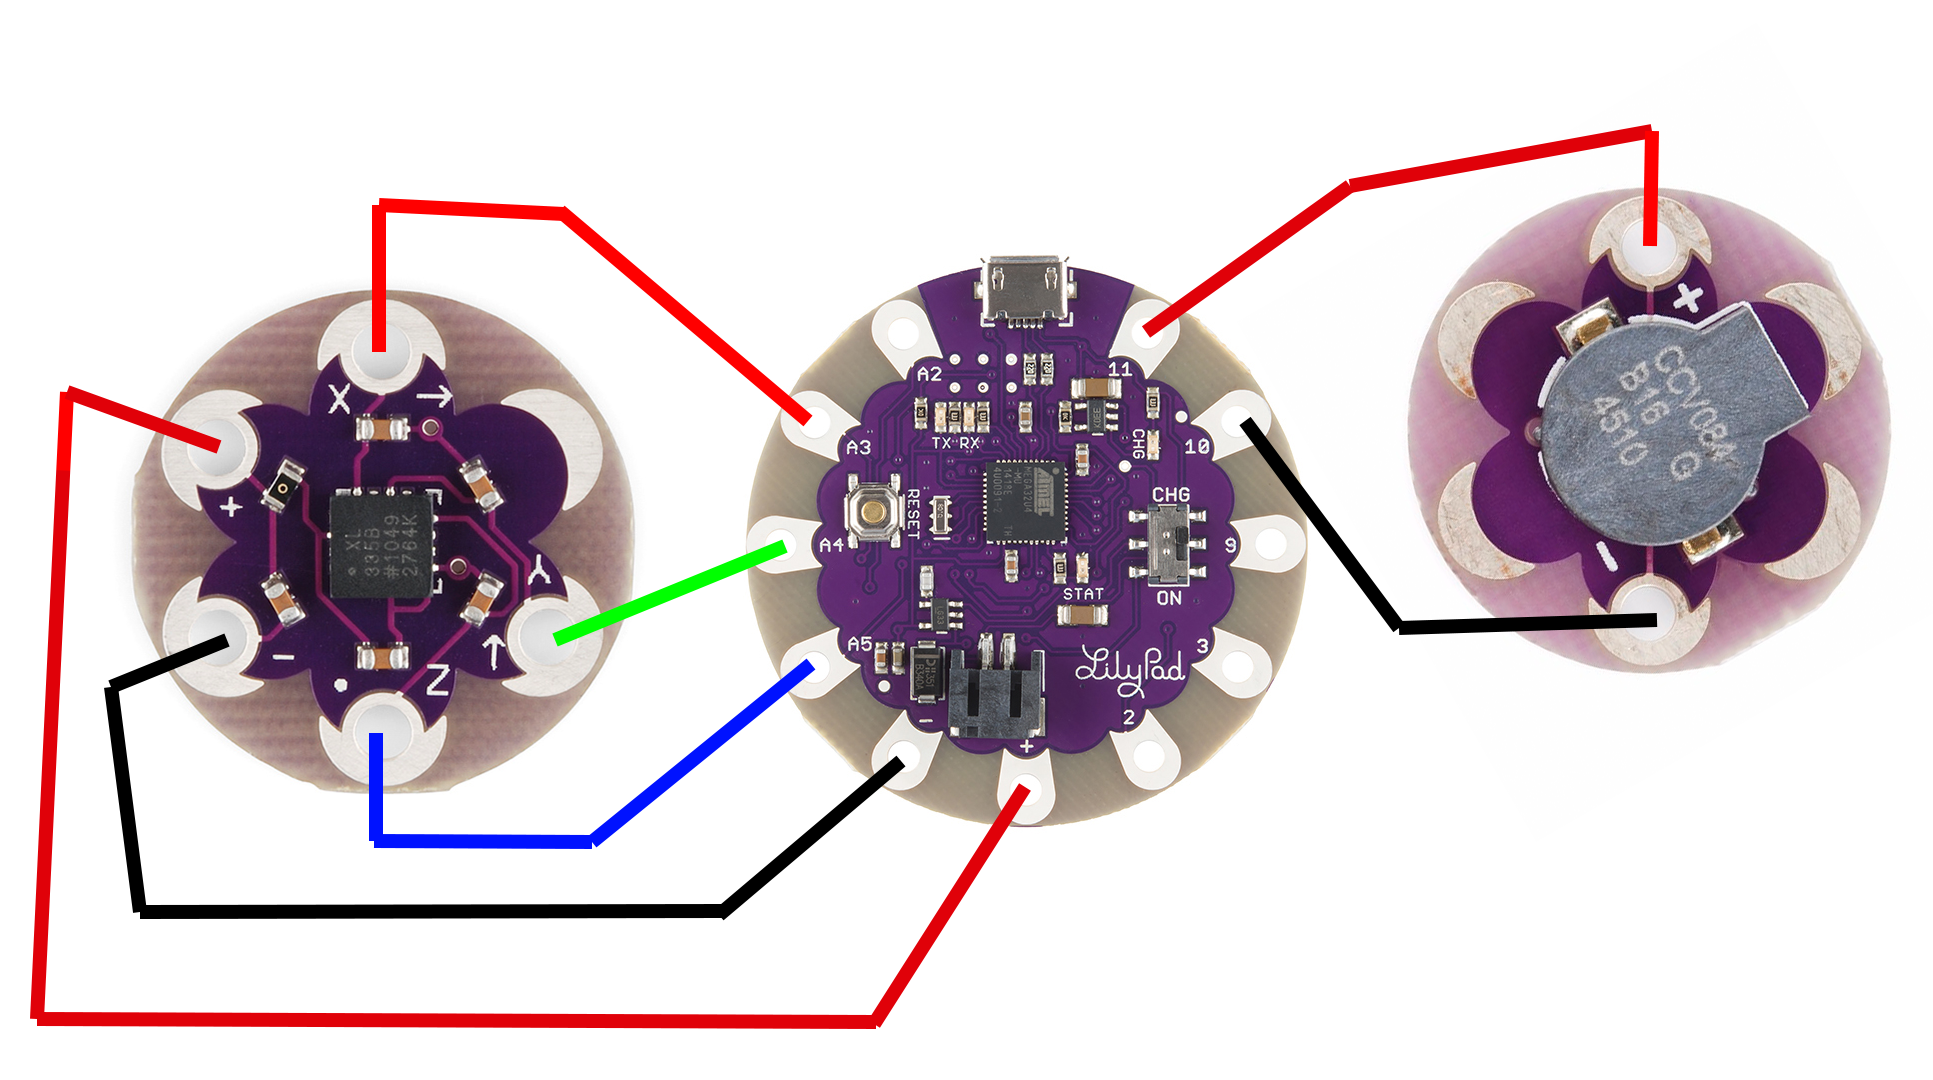
\includegraphics[width=.4\textwidth]{diagrama_conexao.png}
\caption{Arquitetura proposta. O acelerômetro (esquerda), Lilypad USB (meio) e \textit{buzzer} (direita).}
\label{fig:example3}
\end{figure}

O acelerômetro foi costurado perto do pescoço para detectar a inclinação da região. A partir disso, o código, que é executado pelo Lilypad, identifica se a inclinação do pescoço é ou não ideal para a postura em um determinado período de tempo e produzir som através do \textit{buzzer} para notificar o usuário de que sua postura está incorreta.

Sobre o sistema, sãu utilizadas 3 variáveis: postura, \textit{sombuzzer} e \textit{delay}. A postura é o valor de um dos eixos do acelerômetro para verificação da postura do usuário. O \textit{sombuzzer} é uma variável do tipo \textit{int} que representa o volume do \textit{buzzer}. Já a variável \textit{delay} é o intervalo entre os apitos do \textit{buzzer}. Os seguintes conjuntos \textit{fuzzy} são utilizados para avaliação da postura:

\begin{figure}[ht]
    \centering
    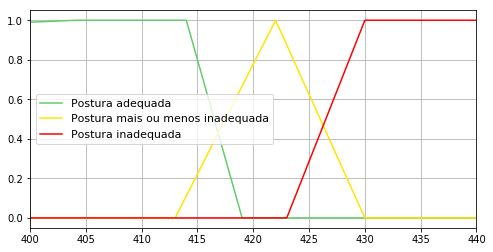
\includegraphics[width=.7\textwidth]{download.png}
    \caption{Conjuntos \textit{fuzzy} para verificação de postura inadequada}
    \label{fig:fuzzy1}
\end{figure}

O sistema de inferência \textit{fuzzy} possui as seguintes regras:

\begin{itemize}
    \item Se a postura estiver MAIS OU MENOS INADEQUADA, então \textit{sombuzzer} é igual a 100 e \textit{delay} é igual a 10;
    \item Se a postura estiver INADEQUADA, então \textit{sombuzzer} é igual a 1500 e \textit{delay} é igual a 50;
\end{itemize}

Para defuzificação, é usado o conjunto \textit{fuzzy} com maior grau de pertinência para obter o valor das variáveis \textit{sombuzzer} e \textit{delay}.

\bibliographystyle{sbc}
\bibliography{sbc-template}

\end{document}
